\chapter{Scheduling}
Un sistema operativo deve allocare diverse risorse tra diversi processi che ne fanno richiesta contemporaneamente. Tra le diverse risorse che i processi possono richiedere, la più ovvia è il processore. Questa risorsa viene allocata tramite lo \textit{scheduling} (pianificazione). 
\begin{redbar}
Quindi lo scopo dello \textbf{scheduling} è assegnare ad ogni processore i processi da eseguire, man mano che i processi stessi vengono creati e distrutti, tenendo conto dei tempi di risposta, del throughput e dell'efficienza del processore.
\end{redbar}

Altri obiettivi dello scheduling sono: distribuire il tempo di esecuzione in modo equo (fair) tra i vari processi; gestire le priorità dei processi quando necessario; evitare la starvation (letteralmente, morte per fame) dei processi; usare il processore in modo efficiente; avere un overhead\footnote{Utilizzato per definire le risorse accessorie, richieste in più rispetto a quelle strettamente necessarie per ottenere un determinato scopo.} basso.

\section{Tipi di scheduling}
Esistono vari tipi di scheduling a seconda della frequenza con cui vengono eseguiti:
\begin{itemize}
    \item \textit{Long-term scheduling} (scheduling di lungo termine), decide l'aggiunta ai processi da essere eseguiti; 
    \item \textit{Medium-term scheduling} (scheduling di medio termine) decide l'aggiunta ai processi che sono in memoria principale; 
    \item \textit{Short-term scheduling} (scheduling di breve termine) decide quale processo, tra quelli pronti, va eseguito da un processore; 
    \item \textit{I/O scheduling} (scheduling per l'input/output) decide a quale processo, tra quelli con una richiesta pendente per l'I/O, va assegnato il corrispondente dispositivo di I/O.
\end{itemize}

Quasi tutte le transizioni degli stati dei processi sono decise dai vari tipi di scheduler (vedi Figura \ref{fig:scheduling-stati}). In particolare, il Long-term scheduling sceglie se un processo appena creato deve essere Ready o Ready/Suspended; il Medium-term scheduling decide tra le versioni di Suspend o non Suspend e viceversa; lo Short-term scheduling si occupa solamente di quei processi Ready, in coda, che aspettano di essere eseguiti.
\begin{figure}[h]
    \centering
    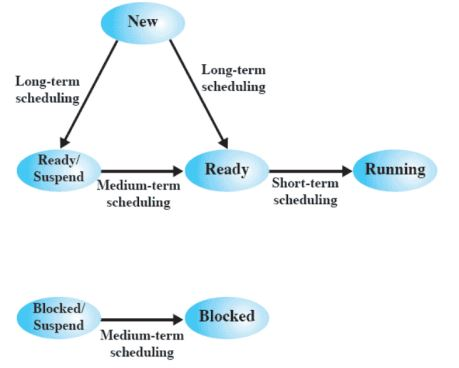
\includegraphics[width=0.44\linewidth]{images/scheduling-stati.JPG}
    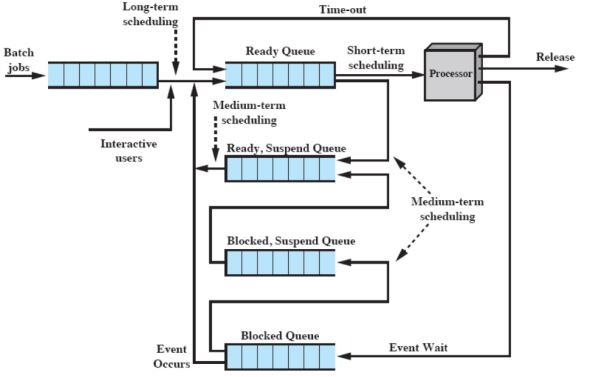
\includegraphics[width=0.55\linewidth]{images/scheduling-code.JPG}
    \caption{Processi e scheduling}
    \label{fig:scheduling-stati}
\end{figure}

\subsection*{Long-term scheduler}
Il Long-term scheduler (LTS) decide quali programmi sono ammessi nel sistema per essere eseguiti. E' di tipo FIFO (First In First Out), ovvero il primo processo in input è il primo ad essere ammesso, e tiene conto dei criteri di priorità, requisiti per l'I/O e tempo di esecuzione atteso. Dato che, il LTS, decide quali processi vanno in RAM, controlla anche il grado di multiprogrammazione.

Quindi tipicamente: i lavori batch vengono accodati e il LTS li prende man mano che lo ritiene "giusto"; i lavori interattivi vengono ammessi fino a "saturazione" del sistema; se si sa quali processi sono I/O bound e quali CPU-bound\footnote{Sono processi che utilizzano molte risorse di I/O o CPU.}, può mantenere un giusto mix tra i 2 tipi, oppure bilanciare le richieste ai dispositivi di I/O. Il LTS può essere chiamato in causa anche quando non ci sono nuovi processi, ad esempio quando termina un processo o quando alcuni processi sono idle\footnote{Tempo durante il quale un mezzo non effettua nessuna attività ed è in attesa.} da troppo tempo.

\subsection*{Medium-term scheduler}
Il Medium-term scheduler (MTS) è parte della funzione di swapping per processi, ovvero del passaggio da memoria secondaria a principale e
viceversa. Questo passaggio è basato sulla necessità di gestire il grado di multiprogrammazione.

\subsection*{Short-term scheduler}
Lo Short-term scheduler (STS), chiamato anche dispatcher, è lo scheduler eseguito più frequentemente ed è tipicamente invocato sulla base di eventi come interruzioni di clock, interruzioni di I/O, chiamate di sistema o segnali.

Lo scopo dello STS è allocare tempo di esecuzione su un processore per ottimizzare il comportamento dell’intero sistema, dipendentemente da determinati indici prestazionali.

\section{Algoritmi di scheduling}
In questa sezione verranno presentati alcuni criteri fondamentali per lo scheduling che possono essere raggruppati in due macro-gruppi:  criteri per l’utente e criteri per il sistema, e criteri prestazionali e non prestazionali.
\begin{itemize}
    \item Il \textit{Turn-around Time} è il tempo tra la creazione di un processo e il suo completamento, comprende anche i vari tempi di attesa (I/O, processore);
    \item Il \textit{Response Time} è il tempo tra la sottomissione di una richiesta e l’inizio della risposta. Lo scheduler deve minimizzare il tempo di risposta medio e massimizzare il numero di utenti con un buon tempo di risposta.
    \item La \textit{Deadline} è utilizzata nei casi in cui si possono specificare scadenze dei processi, mentre la \textit{Predicibilità} richiede che non deve esserci troppa variabilità nei tempi di risposta e/o di ritorno;
    \item Il \textit{Throughput} serve per massimizzare il numero di processi completati per unità di tempo o che abbiano cominciato a produrre output. E' una misura di quanto lavoro viene effettuato che dipende anche dal tempo medio di un processo;
    \item L'\textit{Utilizzo del Processore} rappresenta la percentuale di tempo in cui il processore viene utilizzato;
    \item Con il \textit{Bilanciamento delle risorse}, lo scheduler deve far sì che le risorse del sistema siano usate il più possibile. I processi che useranno meno le risorse attualmente più usate dovranno essere favoriti.
    \item Con \textit{Fairness e Priorità}, se non ci sono indicazioni dagli utenti o dal sistema, tutti i processi devono essere trattati allo stesso modo, se invece ci sono priorità, lo scheduler deve favorire i processi a priorità più alta. Occorrerà pertanto avere più code, una per ogni livello di priorità;
    \begin{figure}[h]
        \centering
        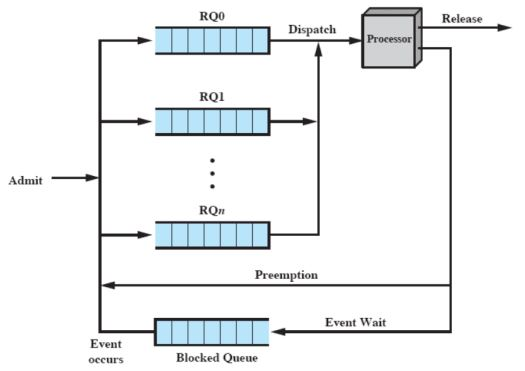
\includegraphics[width=0.5\linewidth]{images/priorita-code.JPG}
        \caption{Code per la gestione delle priorità}
        \label{fig:priorita-code}
    \end{figure}
    \item \textit{Priorità e Starvation}: un processo a bassa priorità potrebbe soffrire di starvation\footnote{Si intende l'impossibilità perpetua, da parte di un processo pronto all'esecuzione, di ottenere le risorse sia hardware sia software di cui necessita per essere eseguito.} a causa di un altro processo a priorità più alta. Una soluzione da adottare potrebbe essere: man mano che l’età del processo aumenta, la priorità cresce.\\
\end{itemize}
In Figura \ref{fig:politiche-di-scheduling} sono presentati i più famosi algoritmi di scheduling con le rispettive caratteristiche. Nei sistemi operativi moderni, generalmente, si utilizzano più combinazioni di questi algoritmi.
\begin{figure}[h]
    \centering
    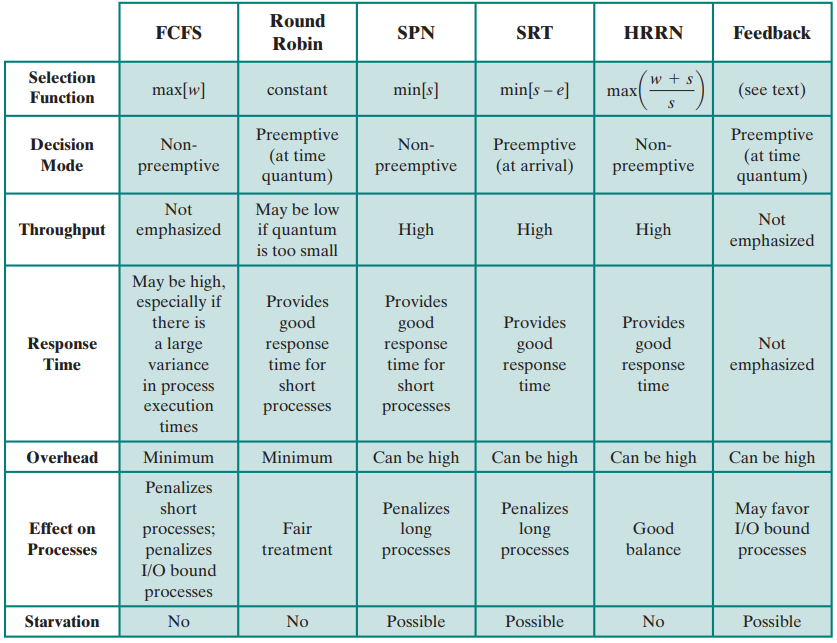
\includegraphics[width=0.7\linewidth]{images/politiche-di-scheduling.PNG}
    \caption{Politiche di scheduling}
    \label{fig:politiche-di-scheduling}
\end{figure}

\begin{itemize}
    \item La \textit{funzione di selezione} è quella che sceglie effettivamente il processo da mandare in esecuzione. I parametri da cui dipende sono: $w$ = tempo trascorso in attesa, $e$ = tempo trascorso in esecuzione, $s$ = tempo totale richiesto, incluso quello già servito ($e$).
    \item La \textit{modalità di decisione} specifica in quali istanti di tempo la funzione di selezione viene invocata. Ci sono 2 possibilità: preemptive o non-preemptive;
    \begin{itemize}
        \item \textit{Non-Preemptive}: se un processo è in esecuzione, allora viene eseguito fino alla sua terminazione o fino ad una richiesta di I/O (o comunque ad una richiesta bloccante);
        \item \textit{Preemptive}: il sistema operativo può interrompere un processo in esecuzione anche se il processo non è terminato o se ci sono delle richieste bloccanti. La preemption di un processo può avvenire o per l’arrivo di nuovi processi (appena forkati) o per un interrupt di I/O.
    \end{itemize}
\end{itemize}

\begin{Example}{Scenario comune di algoritmi di scheduling}{}
    \textit{Supponiamo di avere 5 processi batch divisi come segue:}
    \begin{center}
    \begin{tabular}{|c|c|c|}
    \hline
    \textit{Processo} & \textit{Tempo di arrivo} & \textit{Tempo di esecuzione}\\\hline\hline
         A& 0 & 3\\\hline
         B& 2 & 6\\\hline
         C& 4 & 4\\\hline
         D& 6 & 5\\\hline
         E& 8 & 2\\\hline
    \end{tabular}
    \end{center}
    Vediamo come si comportano i vari algoritmi di scheduling:
    \begin{itemize}
        \item Il \textit{FCFS} (First Come First Served) è non-preemptive, tutti i processi sono aggiunti alla coda dei processi ready e quando un processo smette di essere eseguito, si passa al processo che ha aspettato di più nella coda.

        \begin{minipage}{\textwidth}
            \centering
            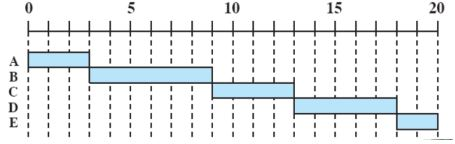
\includegraphics[width=0.5\linewidth]{images/esempio-fcfs.JPG}
            \label{fig:esempio-fcfs}
        \end{minipage}

        Il FCFS favorisce i processi che usano molto la CPU (CPU-bound) ma non è molto efficiente perché un processo "corto" deve attendere molto prima di andare in esecuzione;

        \item Il \textit{Round-Robin} usa la preemption, basandosi su un clock. Talvolta viene chiamato time slicing (tempo a fette), perché ogni processo ha una fetta di tempo.
        
        \begin{minipage}{\textwidth}
            \centering
            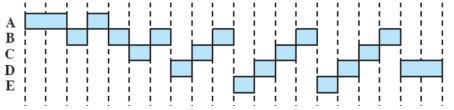
\includegraphics[width=0.5\linewidth]{images/esempio-round-robin.JPG}
            \label{fig:esempio-round-robin}
        \end{minipage}

        Un’interruzione di clock viene generata ad intervalli periodici. Quando l’interruzione di clock arriva, il processo attualmente in esecuzione viene rimesso nella coda dei ready e viene selezionato il prossimo processo. Ovviamente, se il processo in esecuzione arriva ad un’istruzione di I/O prima dell’interruzione, allora viene spostato nella coda dei blocked.

        Con il round-robin, i processi CPU-bound sono favoriti perché usano tutto (o quasi) il loro quanto di tempo, invece gli I/O bound ne usano solo una porzione, fino alla richiesta di I/O. Ne risulta che il round-robin non è equo, oltre che inefficiente per l’I/O. La soluzione consiste nell'implementazione del \textit{round-robin virtuale}, dove dopo un completamento di I/O, il processo non va in coda ai ready, ma va in una nuova coda che ha priorità su quella dei ready, però, solo per la porzione del quanto che ancora gli rimaneva da completare (vedi Figura \ref{fig:round-robin-virtuale}).

        \begin{minipage}{\textwidth}
            \centering
            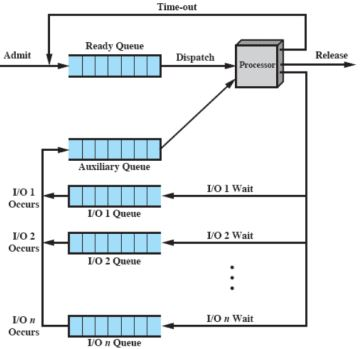
\includegraphics[width=0.5\linewidth]{images/round-robin-virtuale.JPG}
            \captionof{figure}{Round-robin virtuale}
            \label{fig:round-robin-virtuale}
        \end{minipage}

        \item Lo \textit{SPN} (Shortest Process Next) è non-preemptive e prevede che il prossimo processo da mandare in esecuzione è quello più breve, dove per "breve" si intende il processo, tra quelli ready, il cui tempo di esecuzione stimato è minore. Quindi in sostanza i processi corti scavalcano quelli lunghi.

        \begin{minipage}{\textwidth}
            \centering
            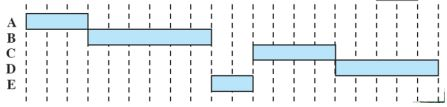
\includegraphics[width=0.5\linewidth]{images/esempio-spn.JPG}
            \label{fig:esempio-spn}
        \end{minipage}

        Con lo SPN la predicibilità dei processi lunghi è ridotta ovvero, è più difficile dire quando andranno in esecuzione perché dipende molto da come si comportano gli altri processi nel sistema. Inoltre, se il tempo di esecuzione stimato si rivela inesatto, il sistema operativo può abortire il processo e i processi lunghi potrebbero soffrire di starvation.

        Per stimare il tempo di esecuzione dei processi si parte dal concetto che in alcuni sistemi ci sono processi (sia batch che interattivi) che sono eseguiti svariate volte. Allora, per questi tipi di processi, si può usare il passato ($T_i$) per predire il futuro ($S_i$). Una prima soluzione può essere svolta attraverso la media dei $T_1,...,T_n$ tempi passati:
        \begin{equation*}
            S_{n+1}=\frac{1}{n}\sum_{i=1}^nT_1\hspace{1cm}S_{n+1}=\frac{1}{n}T_n+\frac{n-1}{n}S_n
        \end{equation*}
        Questa formula, però, dà lo stesso peso a tutte le istanze, quando invece sarebbe meglio far pesare di più quelle più recenti (exponential averaging):
        \begin{equation*}
            S_{n+1}=\alpha T_n+(1-\alpha)S_n\hspace{1cm}S_{n+1}=\alpha T_n+...+\alpha(1-\alpha)^iT_{n-i}+...+(1-\alpha)^nS_1
        \end{equation*}

        \item Lo \textit{SRT} (Shortest Remaining Time) è come lo SPN ma è preemptive. In questo caso l'algoritmo non tiene conto del time quantum, perché un processo può essere interrotto solo quando ne arriva uno nuovo, appena creato. Quindi viene effettuata una stima del tempo richiesto per l'esecuzione, e viene scelto quello più breve.

        \begin{minipage}{\textwidth}
            \centering
            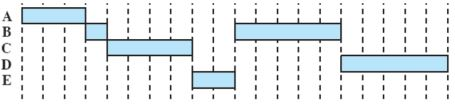
\includegraphics[width=0.5\linewidth]{images/esempio-srt.JPG}
            \label{fig:esempio-srt}
        \end{minipage}

        \item Nel \textit{HRRN} (Highest Response Ratio Next) viene massimizzato il rapporto tra il tempo trascorso in attesa e il tempo totale richiesto dal processo con la seguente formula:
        \begin{equation*}
            \frac{w+s}{s}=\frac{\mbox{tempo trascorso in attesa } + \mbox{ tempo totale richiesto}}{\mbox{tempo totale richiesto}}
        \end{equation*}

        \begin{minipage}{\textwidth}
            \centering
            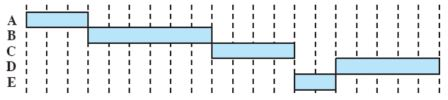
\includegraphics[width=0.5\linewidth]{images/esempio-hrrn.JPG}
            \label{fig:esempio-hrrn}
        \end{minipage}
    \end{itemize}
\end{Example}

\section{Scheduling tradizionale di UNIX}
Nei moderni scheduler, gli algoritmi visti precedentemente non vengono più utilizzati in modo puramente isolato ma si tende a combinare diversi approcci al fine di sfruttare al meglio le caratteristiche specifiche dei diversi algoritmi. Questo è il caso dello scheduling tradizionale di UNIX che combina il concetto di proprietà con il round robin. 
In questo schema, un processo resta in esecuzione per al massimo un secondo, a meno che non termini o si blocchi, e ci sono diverse code, a seconda dei livelli di priorità, dove viene effettuato il round robin. Le priorità vengono ricalcolate ogni secondo e le priorità iniziali sono basate sul tipo di processo: i processi del sistema operativo partono con priorità più alte rispetto ai processi utente.
Per il calcolo delle priorità viene utilizzata una particolare formula, $P_j(i)$ (priority), che indica la priorità del processo $j$ all'inizio di $i$:
\begin{equation*}
    CPU_j(i)=\frac{CPU_j(i-1)}{2}\hspace{1cm}P_j(i)=Base_j+\frac{CPU_j(i)}{2}+nice_j
\end{equation*}
$CPU_j(i)$ rappresenta la misura di quanto il processo $j$ ha usato il processore nell'intervallo $i$, con exponential averaging dei tempi passati, nel caso dei processi running viene incrementato di 1 ogni $\frac{1}{60}s$. Con $Base_j$ si indica il valore iniziale di priorità basato sul tipo di processo e con $nice_j$ un processo può auto-declassarsi come avente bassa priorità.

\begin{Example}{Scheduling in Unix}{}
    \textit{Supponiamo di avere tre processi con $Base_A=Base_B=Base_C=60$ e $nice_A=nice_B=nice_C=0$, vediamo come cambia la priorità durante l'esecuzione dei tre processi.}

    \begin{minipage}{\textwidth}
            \centering
            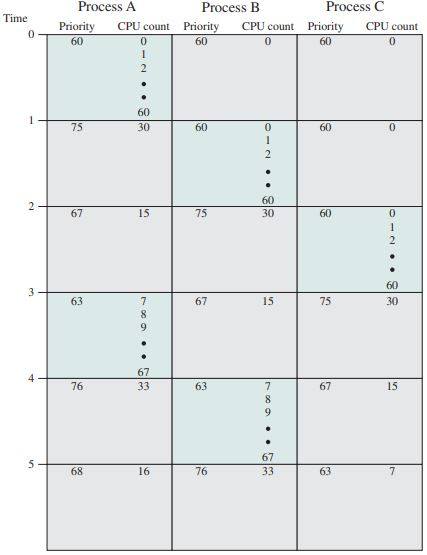
\includegraphics[width=0.5\linewidth]{images/esempio-scheduling-unix.JPG}
            \label{fig:esempio-scheduling-unix}
            \captionof{figure}{Esempio di scheduling in UNIX}
        \end{minipage}

        A partire dal secondo 0 tutti è tre i processi hanno priorità 60 e viene eseguito il processo A che incrementa il suo valore di CPU count fino a 60 (il processo viene eseguito per tutto il quanto di tempo). Quando arriva l'interrupt per la scelta del processo da eseguire vengono ricalcolati, per tutti e tre i processi, i nuovi valori di $CPU_j(i)=\frac{CPU_j(i-1)}{2}=\frac{60}{2}=30$ e $P_j(i)=Base_j+\frac{CPU_j(i)}{2}+nice_j=60+\frac{30}{2}+0=75$.

        Vengono ripetuti questi passaggi per ogni secondo fino alla terminazione dei processi.
\end{Example}

\section{Scheduling su architetture multiprocessore}
Nelle architetture multi-processore e/o multi-core, le singole CPU condividono la RAM e c'è un solo sistema operativo che controlla tutti i processi. In questo tipo di sistemi la scelta del processo da assegnare al processore$_k$ può avvenire per assegnamento statico o per assegnamento dinamico. Nel primo caso quando un processo viene creato, gli viene assegnato un processore fino alla sua terminazione. Si può quindi utilizzare uno scheduler (come quelli visti precedentemente) per ogni processore con il vantaggio di essere di semplice realizzazione e con poco overhead, ma anche con la possibilità che un processore può rimanere idle. Con l'assegnamento dinamico, invece, un processo, nel corso della sua vita, potrà essere eseguito su processori diversi.

\section{Scheduling in Linux}
In Linux si cerca la massima velocità di esecuzione, tramite semplicità di implementazione, per questo motivo non ci sono né long-term né medium-term scheduler. Nel sistema operativo di Linux ci sono delle \textit{runqueues}, sono le code da cui pesca il dispatcher (code dei Ready), e le \textit{wait queues}, sono le code in cui i processi sono messi in attesa quando fanno una richiesta (code dei Blocked).
Al contrario delle runqueues, le wait queues sono condivise tra processori.

Lo scheduling in Linux segue quello di UNIX con il preemptive e la priorità dinamica, a cui vengono aggiunte importati correzioni per essere più veloce possibile e per servire nel modo appropriato i processi real-time. La preemption può essere dovuta a 2 casi: o si esaurisce il quanto di tempo del processo attualmente in esecuzione o un altro processo passa da uno degli stati Blocked a Running.

Linux, inoltre, istruisce l’hardware di mandare un timer interrupt ogni 1ms e quindi il quanto di tempo per ciascun processo è multiplo di 1ms. Per scegliere il valore del quanto di tempo, Linux fa una distinzione tra processi:
\begin{itemize}
    \item I \textit{processi interattivi} (ad esempio azioni con mouse o tastiera) vengono fatti eseguire al massimo dopo 150ms, altrimenti l’utente percepisce una mancata risposta;
    \item I tempi dei \textit{processi batch} (non interattivi) sono personalizzati dallo scheduler in quanto non c'è la necessità di una risposta immediata;
    \item I \textit{processi real-time} (ad esempio riproduttori di audio e video) vengono riconosciuti da Linux solo con un'opportuna chiamata alla system call \verb|sched_setscheduler|.
\end{itemize}

Ci sono essenzialmente tre classi di scheduling: \verb|SCHED_FIFO| e \verb|SCHED_RR| per i processi real-time e \verb|SCHED_OTHER| per tutti gli altri. Verranno eseguiti prima i processi in \verb|SCHED_FIFO| e \verb|SCHED_RR|, poi quelli in \verb|SCHED_OTHER|, infatti le prime due classi hanno un livello di priorità da 1 a 99, la terza da 100 a 139. Quindi ci sono 140 runqueues (una coda con priorità 0 è usata per casi particolari) per ogni CPU.
I processi real-time non cambiano mai la priorità, inoltre un processo \verb|SCHED_FIFO| non viene mai interrotto tranne se si blocca per I/O o se un processo con priorità maggiore passa da uno degli stati Blocked a Running.